% !TEX root = ../featureselection.tex

\vspace*{1em}

\section{INFUSE}
\label{sec:infuse}

In this section, we describe the design of \infuse, which aims to assist predictive modelers with the tasks introduced in Section~\ref{sec:task-analysis}. By providing visualizations for users to interpret the results of feature selection algorithms, as well as the ability to customize the models with domain knowledge that may have been missed by the automated algorithms, \infuse provides a user-centric way of manipulating predictive models.

\begin{figure}[t]
\centering
\hspace*{0.02\linewidth}%
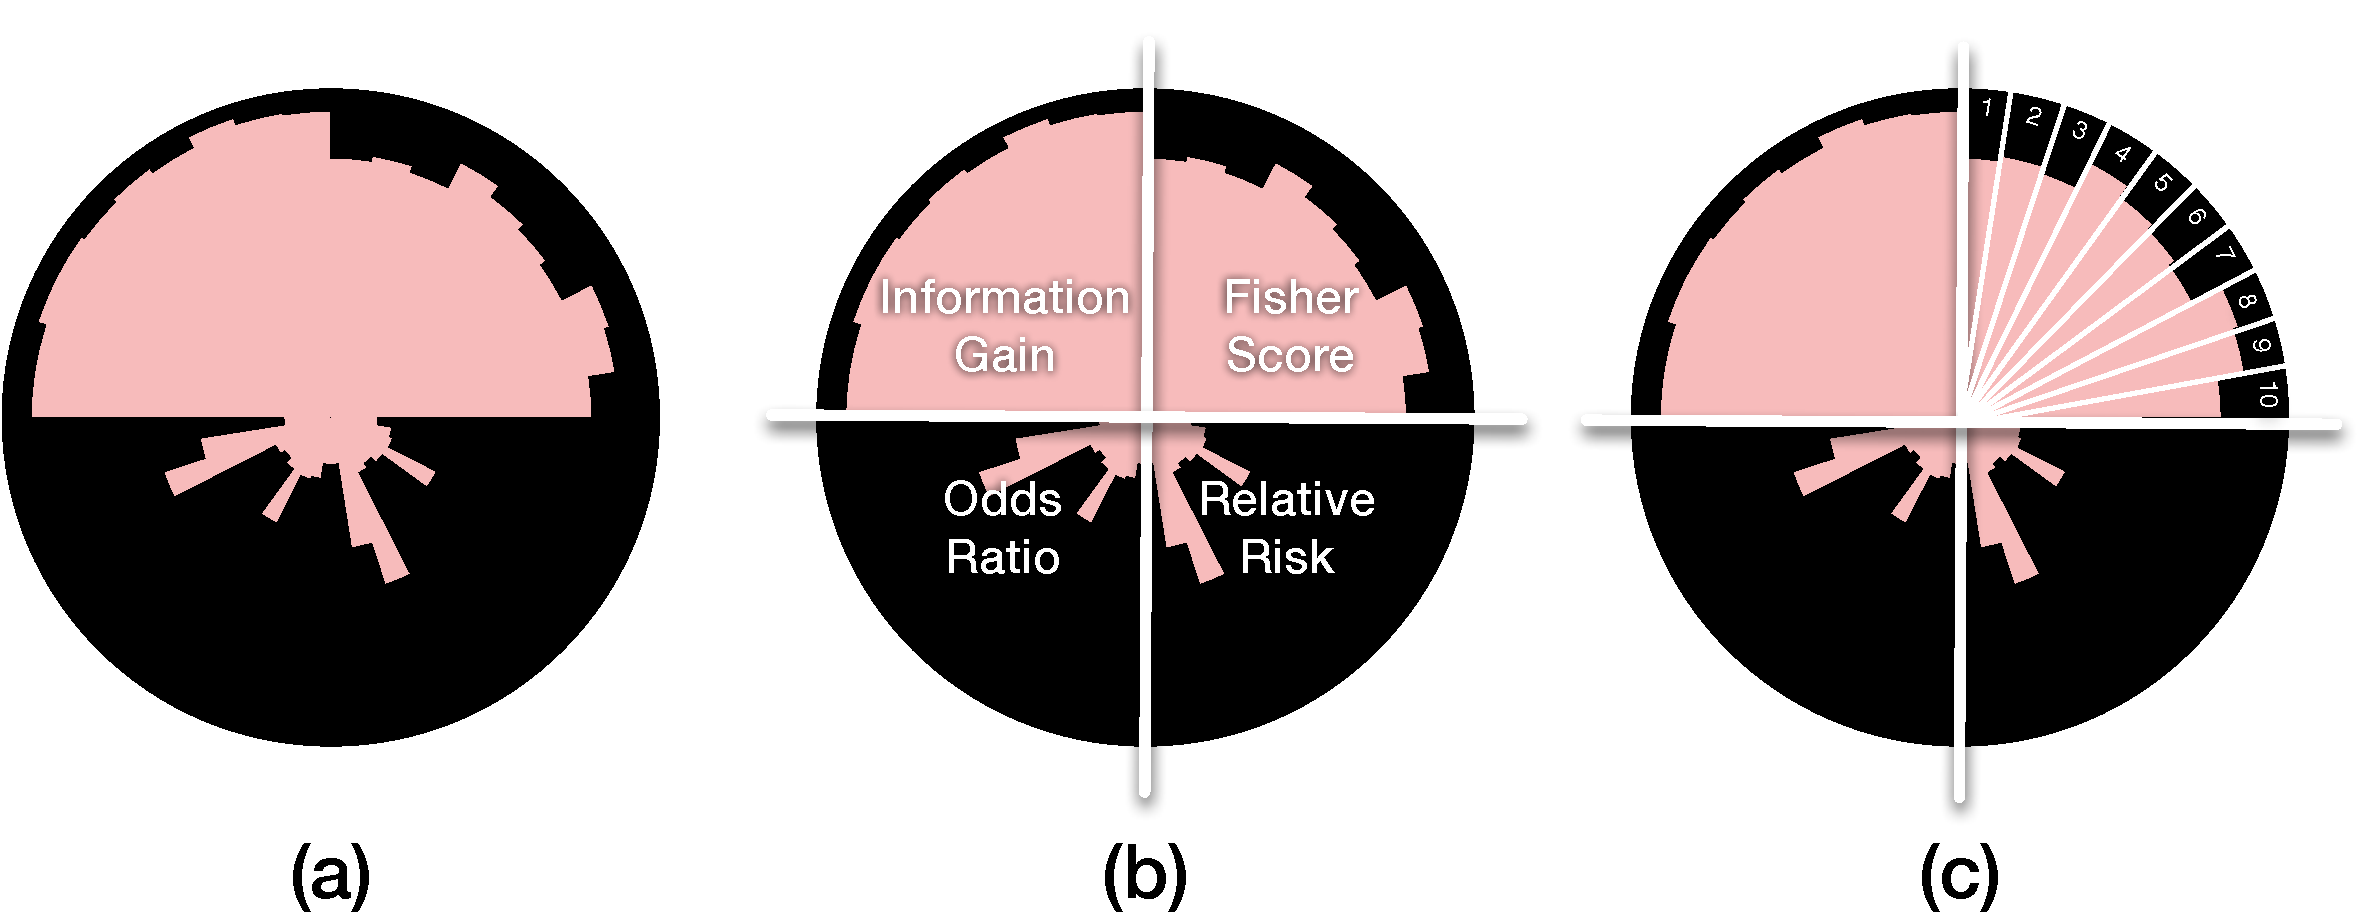
\includegraphics[width=0.95\linewidth]{infuse/glyph-key}
\caption[How to read the glyph representation of \infuse.]{
(a) The glyph representation of a feature in the \infuse system.
(b) Multiple models for each feature are represented as \emph{model sections}.  In this example, the feature is divided into four sections, as it was ranked by four feature selection algorithms (Information Gain, Fisher-Score, Relative Risk, and Odds Ratio.).
(c) Each section is further divided into \emph{fold slices} representing each of the cross-validation folds. Each fold slices features a inward-filling bar that represents the rank of this feature in that fold.
A longer bar implies the feature has a better rank.  If no bar appears, the feature was unranked in the fold, and thus did not meet the importance threshold.
}
\label{fig:glyph-key}
\end{figure}

\begin{figure}[t]
\begin{subfigure}{0.23\linewidth}
\centering
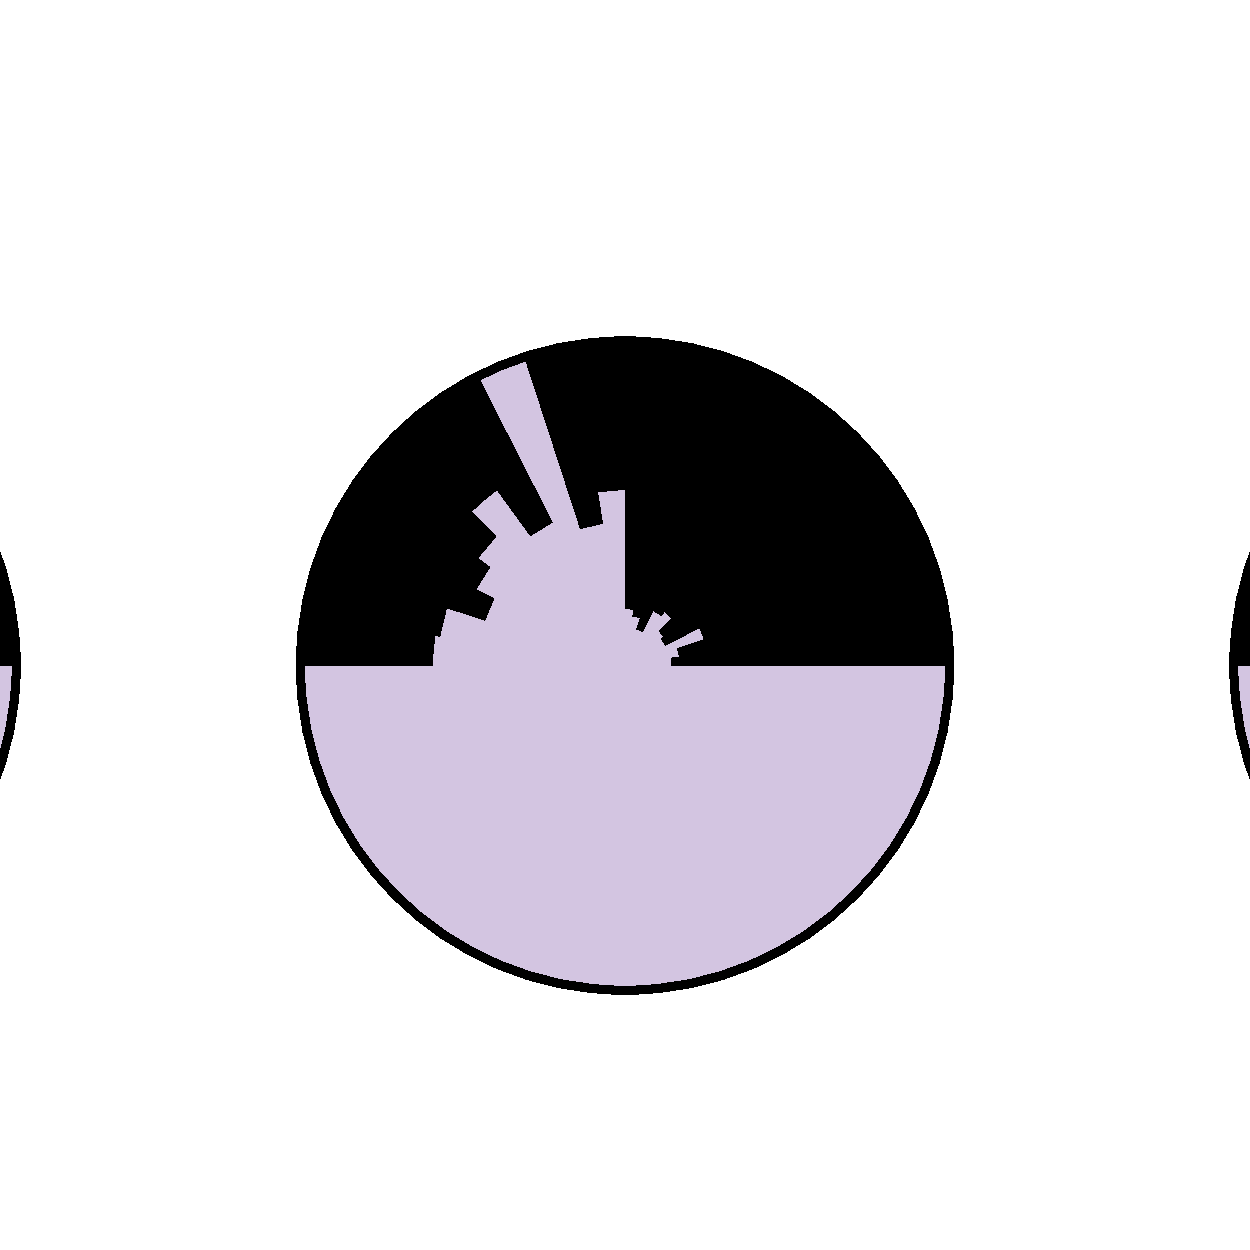
\includegraphics[width=\linewidth,clip,trim={2.4cm 4cm 1.7cm 4cm}]{infuse/g0}
\caption{}
\label{subfig:inward}
\end{subfigure}%
\hspace*{0.01\linewidth}%
\begin{subfigure}{0.23\linewidth}
\centering
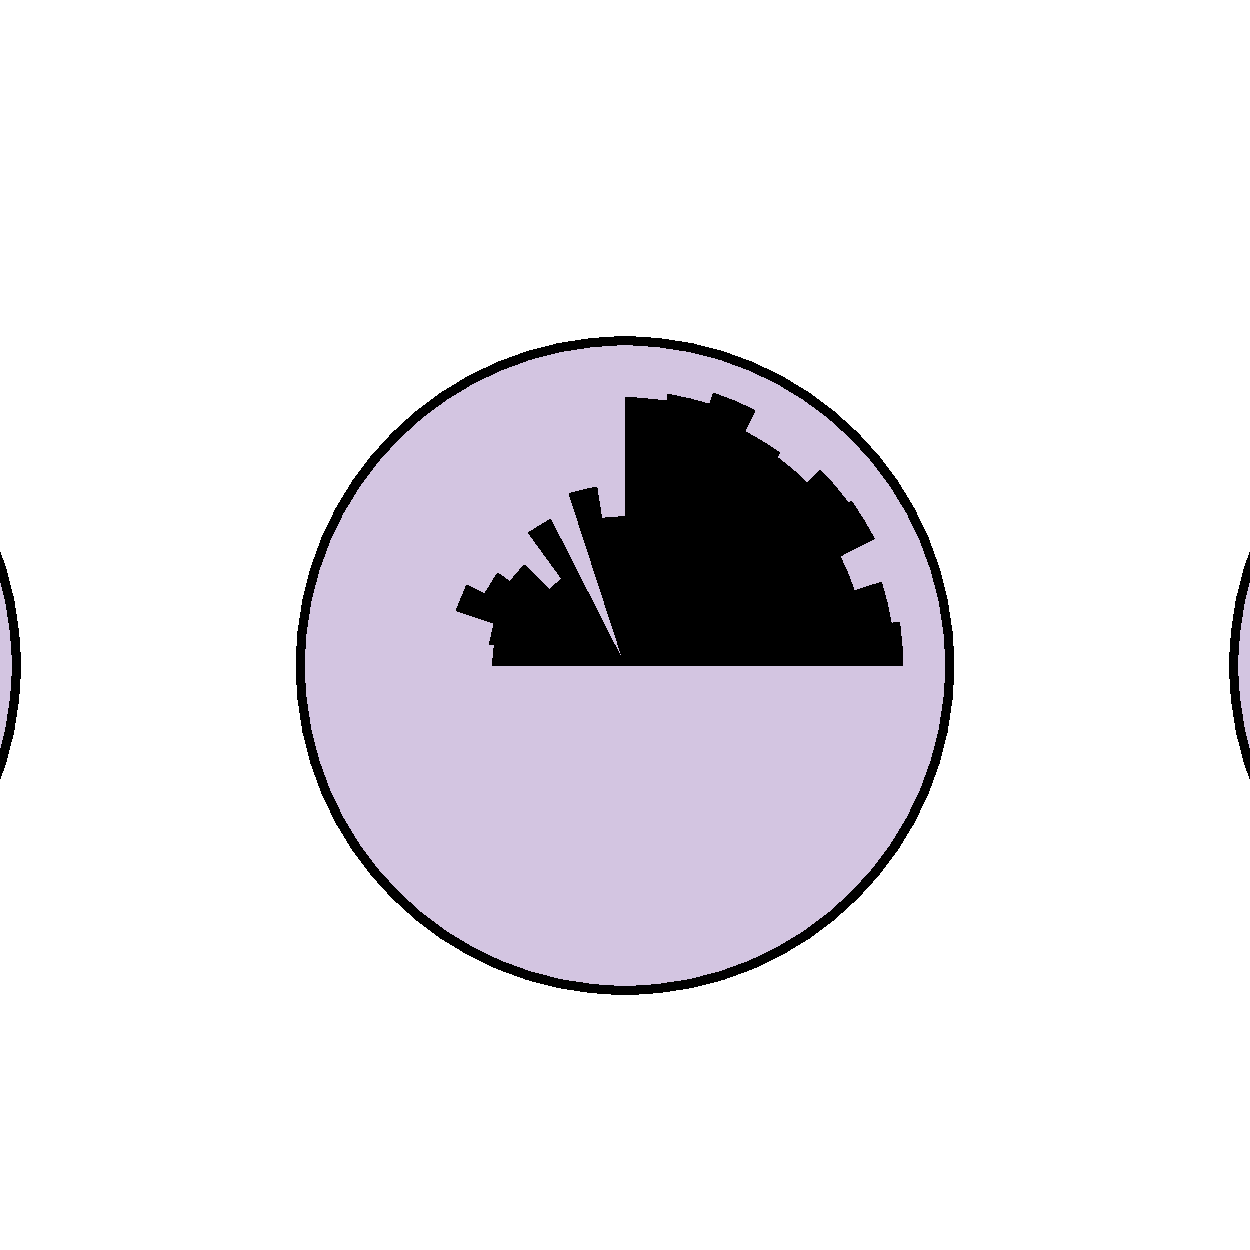
\includegraphics[width=\linewidth,clip,trim={2.4cm 4cm 1.7cm 4cm}]{infuse/g1}
\caption{}
\label{subfig:pie}
\end{subfigure}%
\hspace*{0.01\linewidth}%
\begin{subfigure}{0.23\linewidth}
\centering
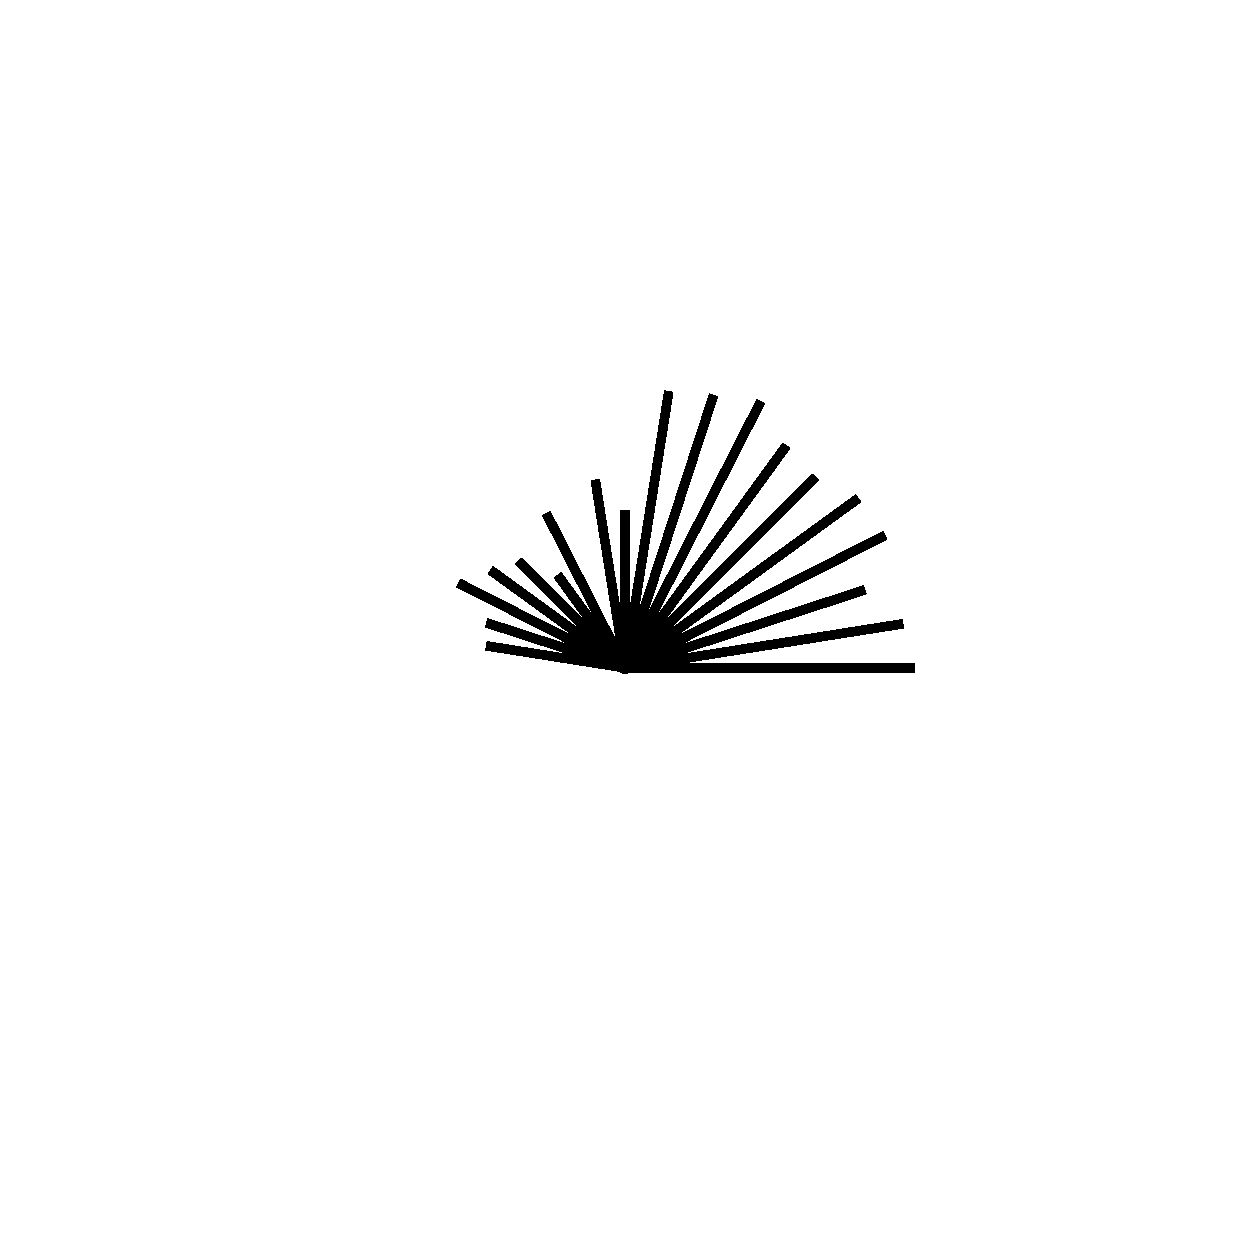
\includegraphics[width=\linewidth,clip,trim={2.4cm 4cm 1.7cm 4cm}]{infuse/g2}
\caption{}
\label{subfig:star}
\end{subfigure}%
\hspace*{0.01\linewidth}%
\begin{subfigure}{0.23\linewidth}
\centering
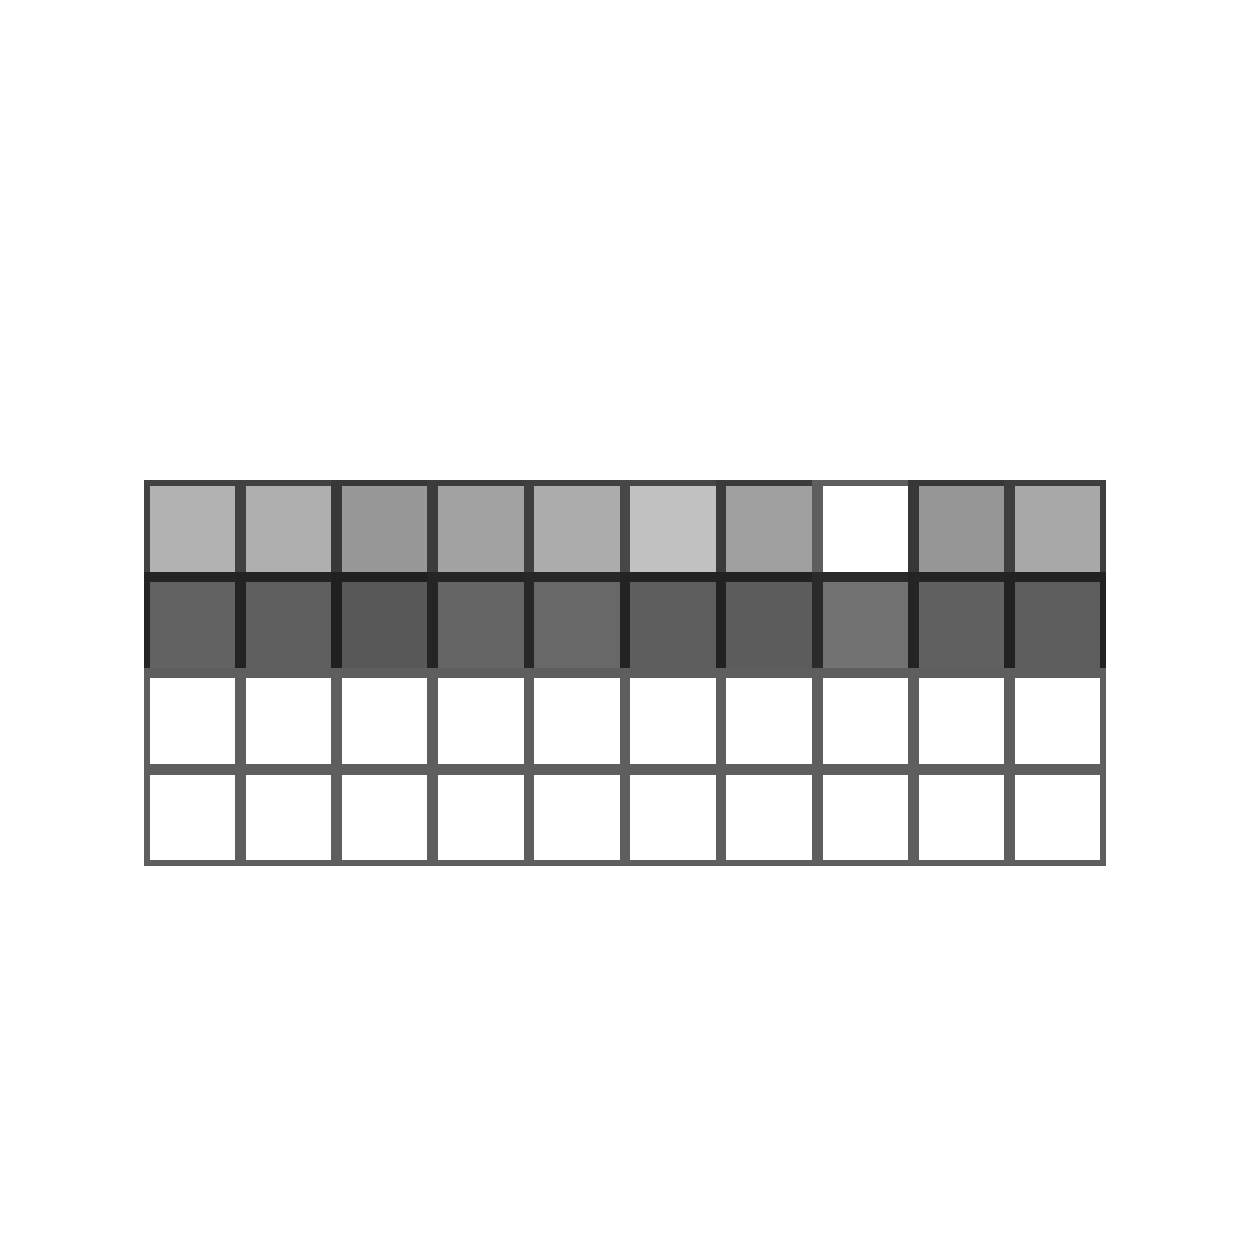
\includegraphics[width=\linewidth,clip,trim={2.4cm 4cm 1.7cm 4cm}]{infuse/g3}
\caption{}
\label{subfig:matrix}
\end{subfigure}%
\caption[Different glyph designs.]{
Different glyph designs.
\subref{subfig:inward} shows \emph{fold slices} with bars growing from perimeter to center
whereas \subref{subfig:pie} grows from center to perimeter.
\subref{subfig:star} shows a typical starburst glyph and
\subref{subfig:matrix} shows a matrix using luminance to show the ranks.
Note that in \subref{subfig:pie} and \subref{subfig:star} it is difficult
to see that this feature is unranked in the third fold from the right in
the top left quadrant.
The values in \subref{subfig:star} are difficult to read because
there is no reference to how big the values are.
Luminance, as used in \subref{subfig:matrix} is a harder perceptual attribute for users
to interpret and distinguish than length and area are, as used by the other glyphs.
}
\label{fig:glyph_design}
\end{figure}

\subsection{Data and Design}

We provide a brief overview of data types utilized by the system. A predictive model, in our setting, is a model trained and validated with machine learning using a high number of features as an input to train the model. These features are the primary data items of \infuse. Each feature has a label representing the feature name (e.g. Diabetes), a category to which the feature belongs to (e.g. Diagnosis), and a subtype (e.g. Problem List, the health problems that led to the diagnosis).

Feature selection algorithms receive as an input the whole set of existing features and return a subset of features selected and ranked according to their estimated predictive power. Since in our setting we use the output of multiple algorithms at once, each feature can further be described by the rankings they receive from all these algorithms (where features that are not selected are marked as unranked). Furthermore, since cross-validation is used, each feature actually gets ranked multiple times by each algorithm, leading to a total number of $\#\textit{feature selection algorithms} \times \#\textit{folds}$ ranks that quantitatively describe each feature.


%As described above in \ref{sec:motivation_healthcare}, feature selection works the features can be ranked by multiple feature selection algorithms, across multiple cross-validation folds. More precisely, for a pre-defined set of feature selection algorithms, each feature can further be described by the which results in number of ranks per feature. If a feature is not selected by a feature selection algorithm, it means it did not reach the threshold to be considered information and is unranked.

The predictive models built using the output generated by feature selection also provide useful information that we use in our system. Each feature set generated by the process described above is used as an input to a classification algorithm. The algorithm builds a model that corresponds to the specific pair of feature set and classification algorithm used for its training. The classifier, in turn, can be described in terms of its performance using the Area Under Curve (AUC), a measure that is commonly used by modelers to give numerical performance scores to models \cite{kuhn2013applied}.

%Each model within a cross-validation fold is then scored by multiple classification algorithms in the form of AUC (the Area Under Curve of the false positive rate in relation to the true positive rate) scores.  The overall quality of a feature set is the average area under curve for all used classification algorithms.

The primary goal of \infuse is to visualize this information so that users can understand the predictive power of features in their models. The user interfaces is organized around three main coordinated views as shown in Figure~\ref{fig:system}: the \textit{Feature View} provides a way to visualize an overview of all features providing information about their attributes and ranking received from feature selection; the \textit{List View} provides a sorted list of all features to get easy access to their labels and to assist the user in searching features according to some predefined criteria like their name or category; the \textit{Classifier View} provides access to the quality scores of each model built using the process described above. The views are coordinated so that selections in one view are propagated to all the other views. In the following we provide additional information about the design of each view.

% Seeing how features perform in various models
% is important for our system.
% Therefore, features showing their ranks in different models are
% first-class citizens of the visualization and for every feature
% the ranks can be seen at any time.
% Features can also be selected by the user to see or build feature sets.
% Selections are linked and visible throughout the tool.

% The system is split into three main components.
% The central part is the feature view that shows all features
% with their ranks as glyphs.
% The positions of the features can be sorted by type and
% overall importance to get an overview or they can
% be positioned on a scatterplot to show additional data about them.
% The type and subtype can be inferred from the glyph.
% Further information about a feature, like name,
% statistics about the rankings which are used as axes for the scatterplot,
% and exact rank numbers can be displayed as tooltip.

% Features are also shown in the list view on the right side.
% This view focuses more on the names of the features but
% shows also the glyph as orientation.
% The order of the elements in the list can be chosen to be by type,
% subtype, and then name, or by showing currently selected features on
% top, ranked by their importance.

% Seeing the area under curve for different
% feature sets is also an important task, since the quality
% of those sets is measured by it.
% In the bottom right corner the area under curve of all models
% is shown for every classification algorithm as matrix.
% Models can be picked to select the features of the corresponding set.

\begin{figure}[t]
\centering
\begin{subfigure}{0.24\linewidth}
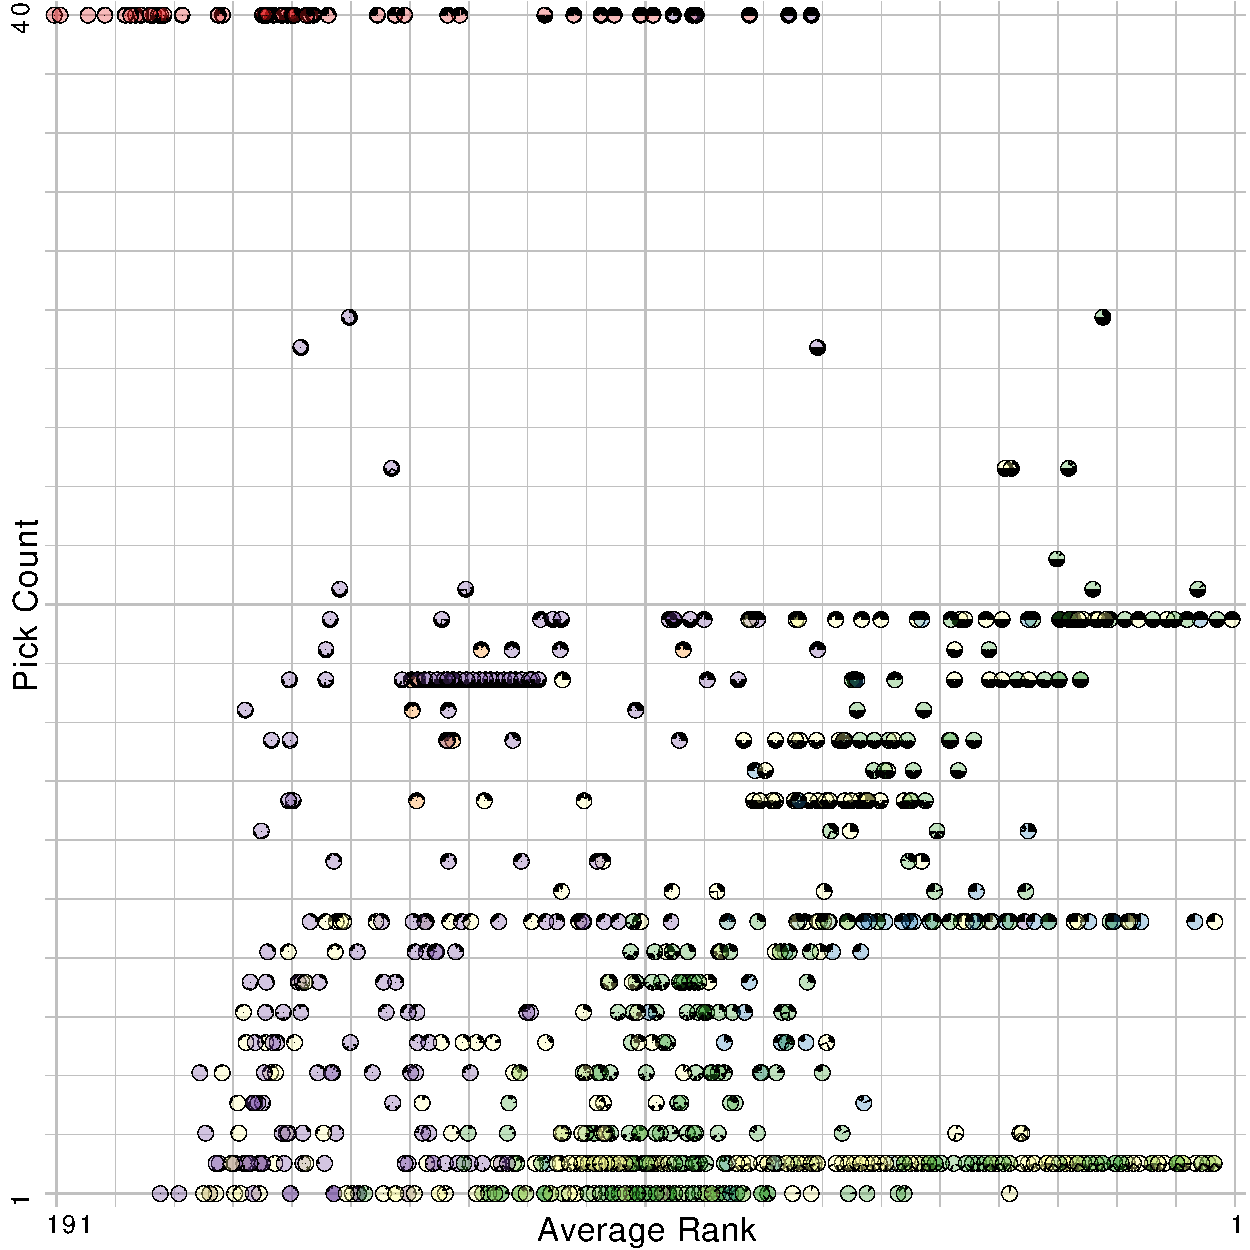
\includegraphics[width=\linewidth]{infuse/ap}
\label{subfig:ap}
\end{subfigure}%
~%
\begin{subfigure}{0.24\linewidth}
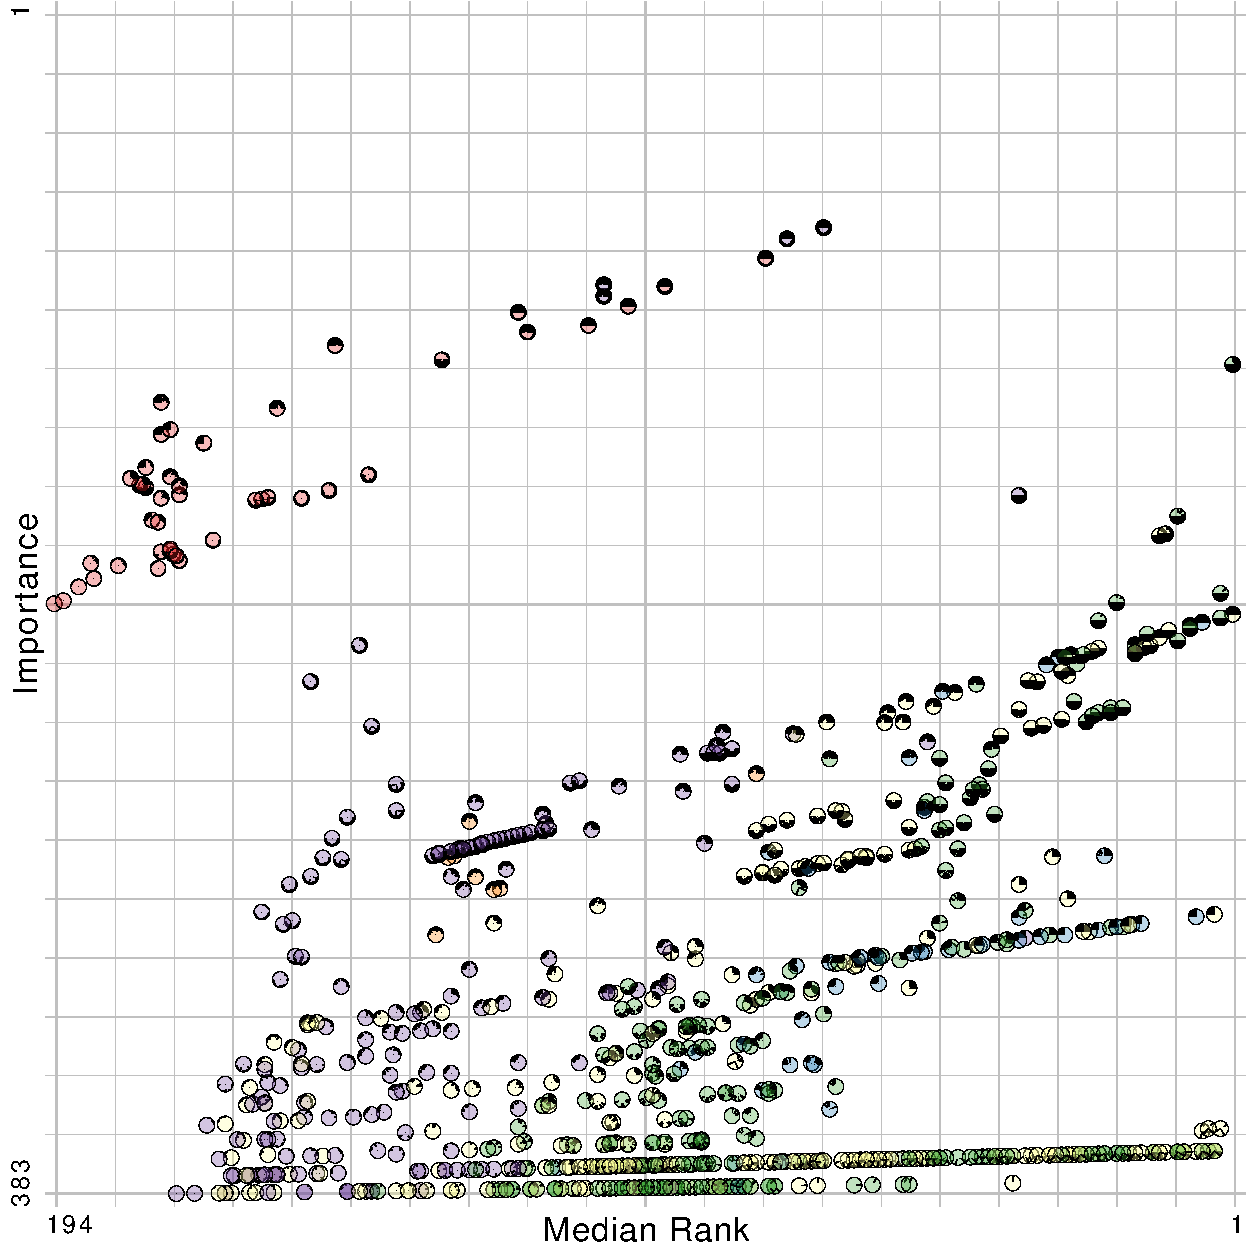
\includegraphics[width=\linewidth]{infuse/mi}
\label{subfig:mi}
\end{subfigure}%
~%
\begin{subfigure}{0.24\linewidth}
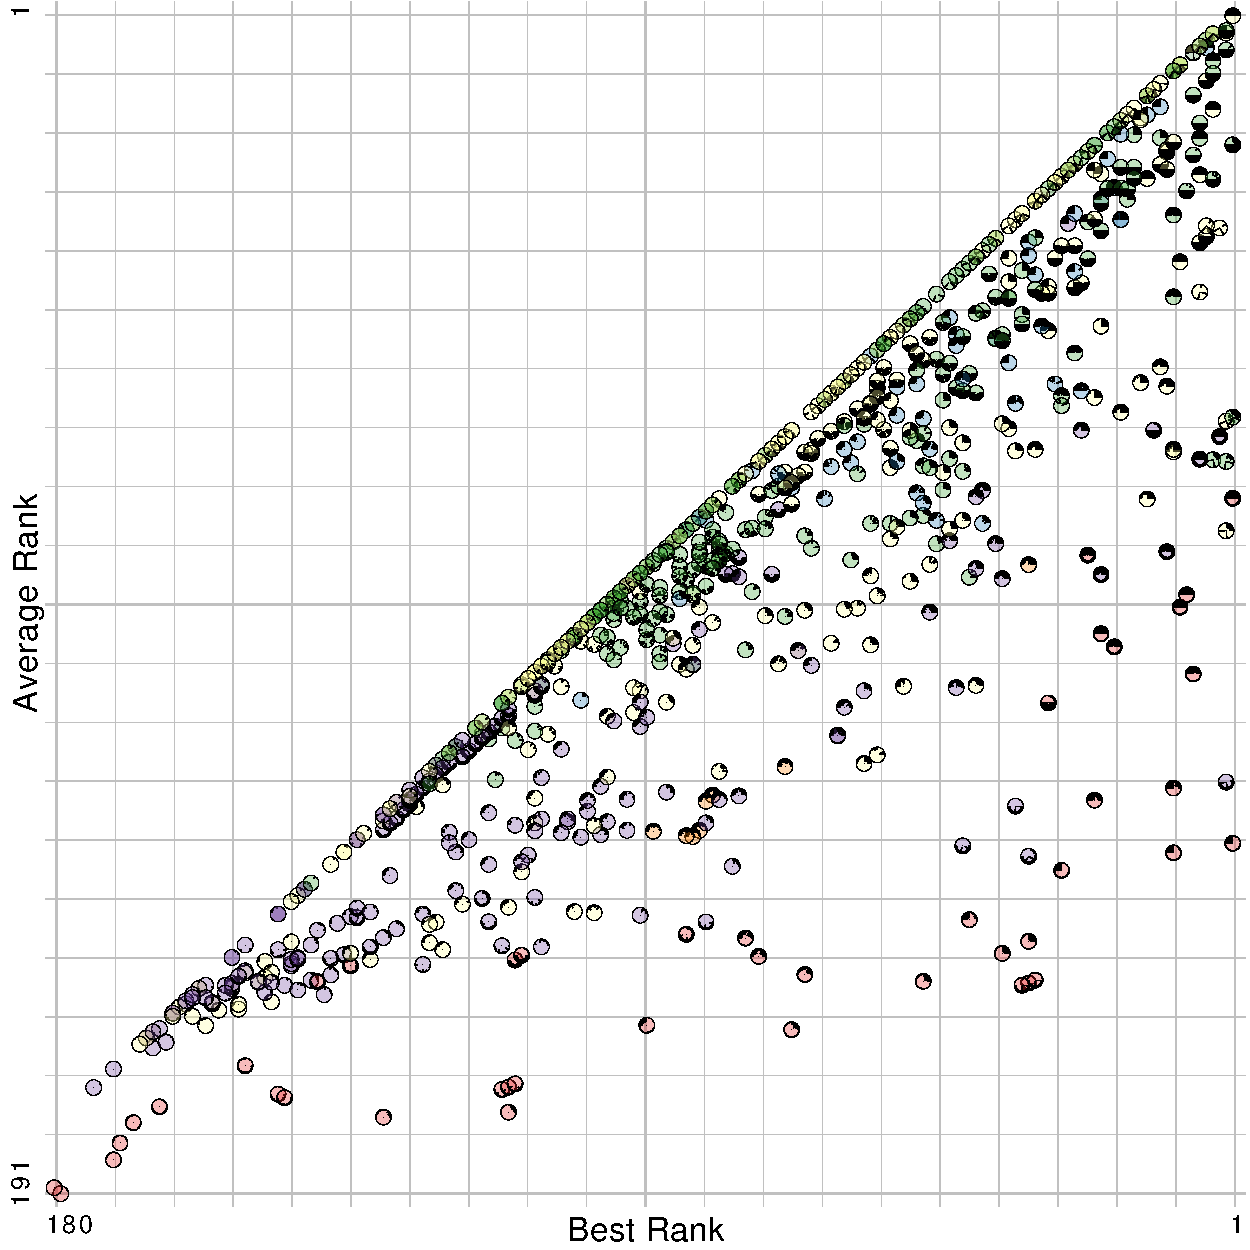
\includegraphics[width=\linewidth]{infuse/ba}
\label{subfig:ba}
\end{subfigure}%
~%
\begin{subfigure}{0.24\linewidth}
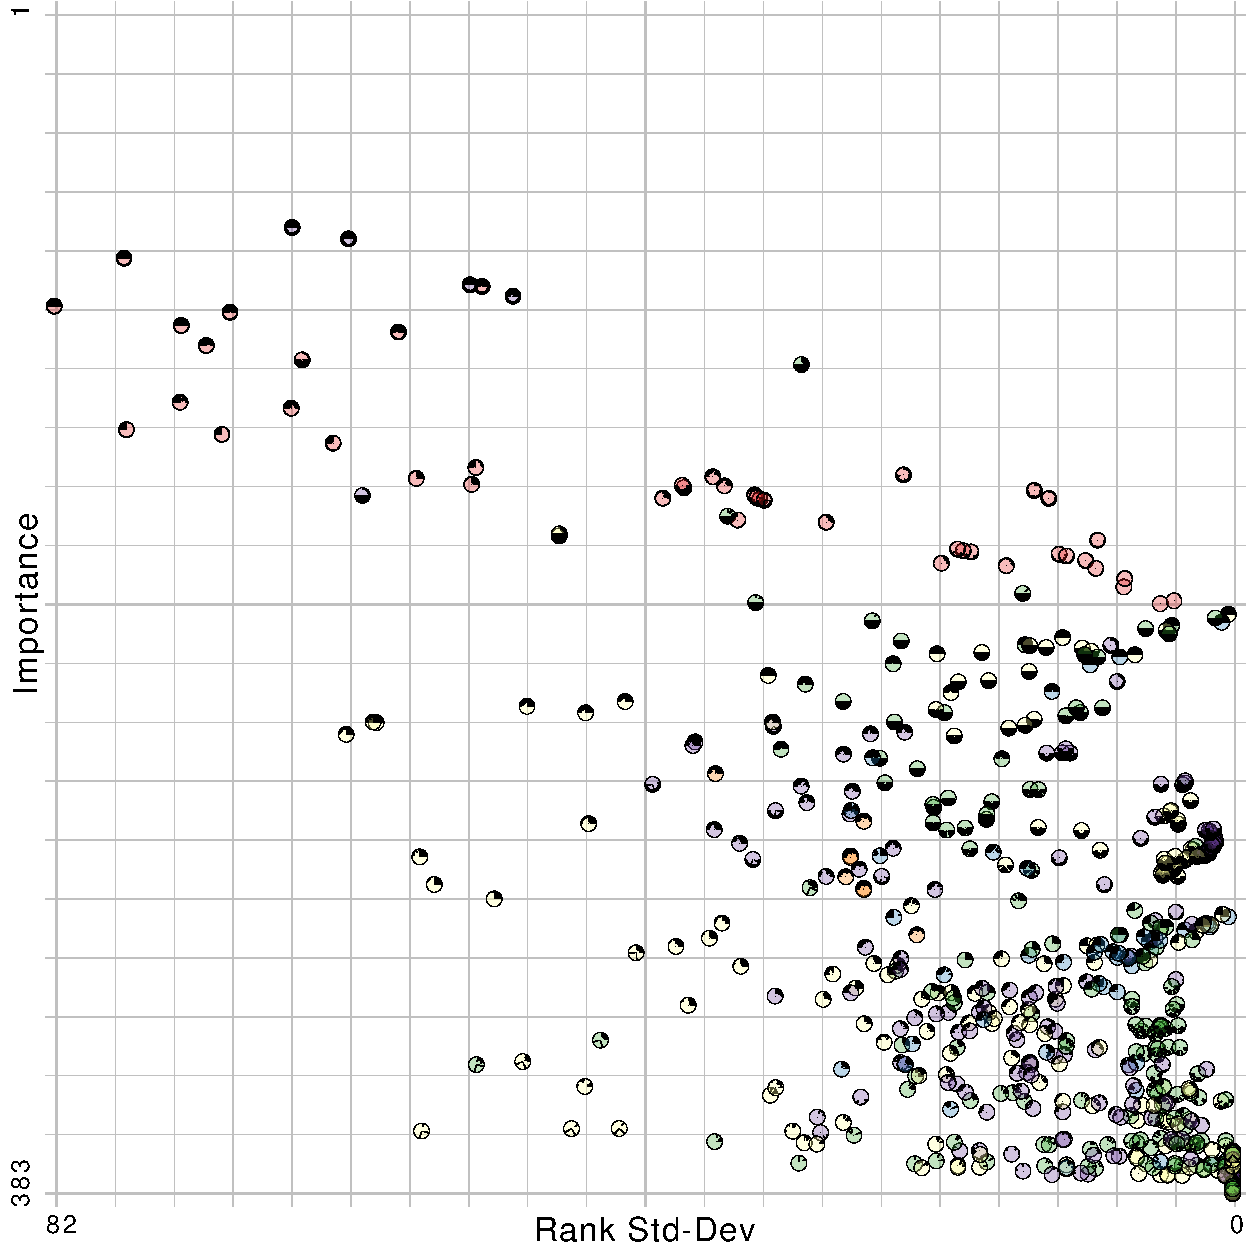
\includegraphics[width=\linewidth]{infuse/si}
\label{subfig:si}
\end{subfigure}
\caption[Different axis combinations for the scatter-plot layout.]{
Different axis combinations for the scatter-plot layout.
In \subref{subfig:ap} the average rank is plotted against the pick count.
Most of the features appear in the lower half because features are rarely picked by more than two algorithms in this example.  The bottom-right shows features that are only chosen
by two models but were ranked very high by them.
\subref{subfig:mi} shows the median rank plotted against the importance.
Notice that the plot looks similar to \subref{subfig:ap} since importance
is a combination of the axes from \subref{subfig:ap}.
The axes in \subref{subfig:ba} are best rank versus average rank.
Features can only appear below the diagonal.
The standard deviation of the ranks is plotted against the importance
in \subref{subfig:si}.
The peak to the bottom right corner consists of features that are rarely
picked and therefore have lower variance.
The peak to the top right consists of features that
are consistently high ranked.
}
\label{fig:scatter}
\end{figure}

\subsection{Feature View}
The primary component of \infuse is the \textit{Feature View}, a zoomable visualization that displays all features as glyphs. Each glyph represents a feature from the original data set and is designed to provide the information outlined above. The main purpose of the feature view is to allow comparison between features and detection of interesting commonalities and differences in terms of how the algorithms rank them. The view allows the user to display the feature set according to two different configurable layouts: a grid layout (the default), which favors legibility, and a scatter plot layout which aims at laying out and grouping the features according to various statistics we collect from the ranks. In the following sections, we describe the design of the glyph as well as the different layouts.

% The design of the glyphs is discussed in Section~\ref{sec:glyphdesign}.
% The glyphs can be laid out in two different ways in the visualization,
% ordered by type and overall importance as described in
% Section~\ref{sec:rankedlayout}, or by positioning them
% on a scatterplot with user defined axes
% (Section~\ref{sec:scatterplotlayout}).
% By clicking on features, the user can toggle its selection.
% A group of features can be selected at once via lasso selection.

\subsubsection{Feature Glyph Design}\label{sec:glyphdesign}
% \adam{on our next phonecall, lets discuss why you call these starburst charts.  there is nothing hierarchical about this data.}
% \adam{note:  low and high ranks are used in misleading ways.  i'm putting this note to make sure we double-check to make sure we're consistent.}
As described in Section \ref{sec:motivation_healthcare}, the features are ranked by multiple feature selection algorithms and across multiple cross-validation folds.  \infuse's glyph design embeds all of this information in a circular glyph that shows all the rankings obtained from each algorithm/fold pair. As shown in Figure~\ref{fig:glyph-key}(a), the glyph is divided into equally-sized circular segments; where each segment represents one of the ranking algorithms.
For instance, in Figure \ref{fig:glyph-key}(b), since the feature was ranked by four feature selection algorithms, the circular glyph is divided into four sections. Each of these sections are then divided further into a \emph{fold slice} for each cross-validation fold. For instance, in Figure \ref{fig:glyph-key}(c), each feature selection algorithm was executed on 10 cross-validation folds, therefore there are 10 fold slices.

Within each fold slice, there is an inward-growing bar (that is, starting from the perimeter and growing towards the center) that represents the rank of the feature in a particular fold. For example, in Figure \ref{fig:glyph-key}(c), the feature is higher ranked in Fold 3 than in Fold 4 as the bar in Fold 3 stretches closer towards the center than in Fold 4. Features that are unranked, because their scores are too low to meet the minimum threshold requirement of the algorithm, are represented as empty slices with no bars. We designed fold slices with inward-growing bars on purpose to help distinguishing between slices with empty values from those with low values. During our design iterations we realized in fact that outward pointing bars would make this distinction too hard to make. Since the information of whether a features is picked up by an algorithm is crucial for its interpretation we decided to opt for this design.

%this way on purpose to have bars growing from the perimeter to the center of the circle so that folds with poor ranks can be easy detected since a fold slice has greater area closer to the perimeter.  This makes it possible to identify the basic properties of a feature selection model even when the interface is zoomed-out.



% Features are shown as inward growing starburst pie chart glyphs showing their ranking in the different models. Each pie slice represents one model. The better the rank of the feature the more the slice expands towards the center of the glyph \emph{ie.} when the feature is ranked as number one by the model the corresponding slice has the same radius as the glyph.
% If the feature is not ranked by the model the slice is not shown.
% Letting slices grow from the outside to the inside makes
% low ranks easier to read since a pie slice has a greater area at the outside.
% This enables to see low ranks and identify their model even when
% the visualization is zoomed out.
% For pie slices growing towards the outside it is difficult to
% identify the model when a rank is low.
% Consider a feature that is ranked very low in only one
% model and unranked in the other models.
% When zoomed out only a dot in the center of the glyph is visible.
% This dot could grow in any direction representing any model.
% Also, as shown in Figure~\ref{fig:glyph_design},

% Figure \ref{subfig:pie} shows an example of a glyph where the fold slices grow from the center towards the perimeter. From the figure one can see that distinguishing empty values is harder with this solution than the one we selected.

%Consider the situation where there is a lowly-ranked feature only ranked in one fold slice section.  When zoomed-out, the glyph would just appear as a circle with a dot in the center, and the user would not know which model or fold ranked the feature.

%Furthermore, it is difficult to see in which fold a feature is unranked when the surrounding models rank the feature.

Multiple glyph designs were considered and tested within \infuse.  For instance, Figure \ref{subfig:pie} shows an example of a glyph where the fold slices grow from the center towards the perimeter.
This makes it difficult to identify fold slices with poor ranks.
Consider the situation where there is a lowly-ranked feature only ranked in one fold slice section.  When zoomed-out, the glyph would just appear as a circle with a dot in the center, and the user would not know which model or fold ranked the feature.  Furthermore, it is difficult to see in which fold a feature is unranked when the surrounding models rank the feature.  Other glyph designs that were tried involve a star glyph (Figure \ref{subfig:star}) and a matrix glyph (Figure \ref{subfig:matrix}).  The star glyph was less effective as users were not afforded a reference point for the maximum ranking and the design leads to some visual artifacts (like high density in the center and lower density in the outer part).
The matrix glyph was less effective, as perceiving differences is more difficult when using luminance than length and area as we do in our final design.

%Furthermore, both of these charts were also less suited for a zoomable user interface than the chosen design.

Users can gain more details about each section and slice by hovering over the region of interest to view an informative tooltip. Furthermore, an overview key is available to remind users of the position of each model type. The background color of the glyph corresponds to the subtype of the feature and a color key can also be shown as a reference to remember the meaning of the color coding (see bottom-left corner of Figure~\ref{fig:system}).

% Pie slices are ordered by feature selection
% algorithm first and then by fold.
% This groups all results from one feature selection algorithm together
% and creates quadrants which can be used for reasoning.
% A key for those quadrants can be shown in the visualization
% and when hovering a slice with the mouse the identity of the model
% and the rank is shown in the tooltip.

% A circle with the radius of the glyph is drawn to distinguish glyphs
% from each other and defines the value bounds.


% Using colors to show ranks, for example as cell colors of a
% feature selection algorithm by fold matrix,
% is not as easy to read as the presented glyph.
% Also, normal starburst glyphs do not work very well when the
% visualization is zoomed out as the lines become thinner and harder to see.

\subsubsection{Ranked Layout}\label{sec:rankedlayout}
The first layout available to users is the ranked layout, which arranges glyphs by their feature type, and sorts them by their overall importance.  The name of the feature type is shown at the first position in the group, after that the features are laid out row-first in a grid-like manner, as shown in Figure \ref{fig:system}. This space-filling approach results in features that are always visible without overlaps.

Features within a group are sorted by their importance. Importance is computed as average rank with
penalized unranked features:
\[
rank_{best} = \min_{m \in M \times V, f \in F}{[rank_{m}(f)]}
\]\[
i(f) = \dfrac{1}{| M \times V |}[
2 \cdot rank_{best} \cdot
unranked_{M \times V} (f)
+ \sum_{m \in M \times V} rank_{m}(f)
]
\]
where $M$ is the set of models, $V$ is the set of cross-validation folds,
$F$ is the set of features,
$rank_{m}(f)$ is the rank of a feature $f$ in the combined model
and cross-validation fold $m$,
and $unranked_{M \times V} (f)$ is the number
of such combined models that did not choose $f$.
Assume $rank_{m}(f) = 0$ for unranked features $f$
in the combined model $m$ only when computing $i(f)$.
Note that a small value for $i(f)$ means higher importance.
The optimal value is $1$.

\subsubsection{Scatterplot Layout}\label{sec:scatterplotlayout}
The second layout available to users is the scatterplot layout, where users can select choices for both axes of the scatterplot.  The choices for axes include:

\begin{itemize}
\item the \emph{average rank} of a feature\\
(ignores unranked folds and models)
\item the \emph{pick count} of the number of combined
models\\and cross-validation folds that picked the feature
\item the \emph{importance} of a feature (defined above)
\item the \emph{best rank} of the feature
\item the \emph{median rank} of the feature\\
(ignores unranked folds and models)
\item the \emph{standard deviation} of the feature's ranks\\
(ignores unranked folds and models)
\end{itemize}

By default, the average rank is chosen for the horizontal axis and
the pick count is chosen for the vertical axis, as shown in Figure \ref{fig:usecase2}.  This combination of axes led to the most insights during the case studies.  However, if users choose to select different axes or pivot to a different layout, animation is used for the transition.  By using slow-in and slow-out animation, users are given time to anticipate the movement direction of the feature, and are able to track features during the transition easily.

% The combination of those axis contents give the most insights.
% The values of the axes are mapped from the
% minimum to the maximum value.
% The lower left corner of the scatter-plot is consistently the
% worst values of both axis and the top left corner is always the best
% values of both axis contents.

\subsubsection{Interaction}
The Feature View provides a number of interactions.
Zooming and panning enables a user to get an overview of the
displayed data and focus on the details of a small number of glyphs.  This exploration can be reset by clicking on the
``Reset View" button, or double clicking on the background. Double clicking on a feature glyph zooms in on the feature so that it fills the viewport.
In addition, a tooltip is shown when a user hovers the mouse
over a glyph. This tooltip provides information about the name, type,
and subtype of the represented feature, as well as all of the statistical
information used for the scatterplot layout. Hovering over a fold slice
in the glyph gives further information about the feature selection algorithm,
the cross-validation fold, and the feature's rank in question.  In order to select features for interactive model building
(see Section~\ref{sec:imb}) the user can click on glyphs to toggle
the selection or use a lasso gesture to select a group of features.
As mentioned in the previous section, users can change the
layout of the glyphs with the buttons below the Feature View.

\subsection{List View}
A simple yet important view of features is the List View, which provides a sorted list of all features, useful for selecting features by name.  Each list item contains the name of the features along with its glyph.  The selection of a feature can be toggled in the list by clicking its list item.  As the selection of features is linked between views, this sorted and labeled view supports users finding particular features of interest and highlighting them in the complementary views.

The list view can be sorted in a few different ways. By default, features are first sorted by
the type of the feature, then by its subtype, and finally by its name.  Users can also sort the list by selection, which means currently selected features are displayed at the top and the unselected features appear after them.  Within these groups, the features are then sorted by their importance.

In addition to sorting, a user can filter the list view via the search box on
the top.
Search terms are separated by white-spaces and the list view
shows all features that contain all search terms in the name, type, or
sub-type.
The results are ranked by the sum of the inverse positions
of the search terms within the feature description.
This favors terms occurring at the beginning of the feature's name
and terms that occur multiple times in one feature description
(see the top right panel of Figure~\ref{fig:system} for an example query).

\begin{figure}[t]
\centering
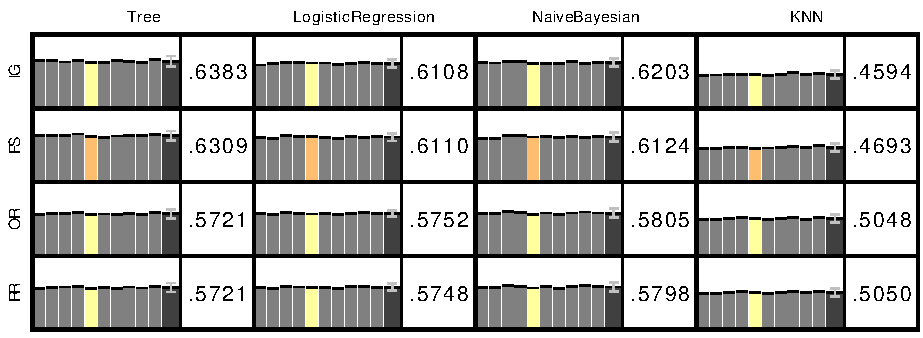
\includegraphics[width=0.7\linewidth]{infuse/classifier}
\caption[The Classifier View.]{The Classifier View displays the results of the classification algorithms for all models.
Rows represent feature selection algorithms and columns represent classification algorithms.
A more detailed description of the cells can be
seen in Figure~\ref{fig:classifier-cell}.
The currently selected model is highlighted in orange, and the results for the same fold in different
feature selection algorithms are highlighted in yellow.  When users select a model, the features that make up the model are highlighted in the Feature and List views.
}
\label{fig:classifier}
\end{figure}

\subsection{Classifier View}

The Feature View and the List View both focus on supporting users to interpret the rankings of features across multiple predictive models.  However, it is also important for users to understand the quality of each model in predicting the appropriate outcome.  The Classifier View, shown in the bottom-right panel of \infuse, is where the quality of each the predictive models can be analyzed.

Typically, predictive models are evaluated using classification algorithms which provide an AUC score (area under ROC curve,
the sensitivity as function of the false positive rate).  Perfect models will have an AUC score of 1, whereas random guessing will have an AUC score of 0.5.  The Classifier View was designed to show AUC scores for each model and fold.

\begin{figure}[t]
\centering
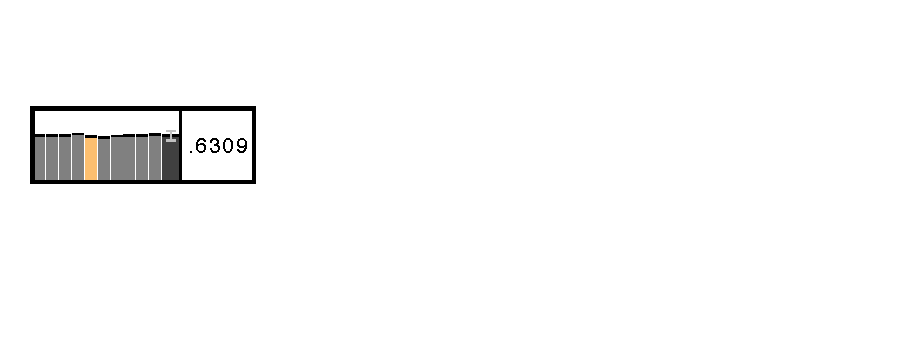
\includegraphics[width=0.4\linewidth]{infuse/classifier-cell}
\caption[A cell of the Classifier View.]{
Each cell in the Classifier View represents the scores of a particular model by a particular classifier.
On the left, there is a bar for each of the validation folds.  The height of each bar corresponds to the AUC score for each fold.  Immediately to the right of the fold bars, the thicker and darker bar and its height represents the average value across all folds.  This bar also features an error bar depicting the standard deviation across the folds.  Finally, to the right of the bars, there is a numerical representation of the average AUC score.}
\label{fig:classifier-cell}
\end{figure}

As illustrated in Figure \ref{fig:classifier}, each row of the Classifier View represents the predictive model that resulted from each feature selection algorithm.  Each column represents a classification algorithm.  Multiple classifiers are used because there are a variety of techniques to evaluate models, and in order to avoid biases, \infuse provides the ability to compare the output from multiple classifiers.

Each cell, as shown in Figure \ref{fig:classifier-cell}, has several components.  On the left, there is a bar for each of the validation folds.  The height of each bar corresponds to the AUC score for each fold.  There is also a slightly thicker and darker bar immediately to the right of the fold bars, and its height represents the average value across all folds.  This bar also features an error bar depicting the standard deviation across the folds.  Finally, to the right of the bars, there is a numerical representation of the average AUC score.  As this information is important for predictive modelers to reason about the quality of models, these values are given visual prominence. The bars, however, can be used to also reason about the quality across all folds.

% A matrix showing feature selection algorithms as rows and
% classification algorithms as columns shows those values.
% Each cell is divided into two parts.
% The first part splits the averaged result for one feature selection
% algorithm into the results of the underlying folds.
% The areas under curve for all folds are shown as bar charts.
% The average area under curve for this
% pair of feature selection and classification algorithm is shown
% as slightly thicker and darker bar on the right end of the bar chart.
% An error bar depicts the five times amplified standard deviation
% over the folds.
% The second part shows the average area under curve as actual number.
% This is important for users to be able to directly reason about the values.

Rows are sorted by the average AUC scores across all classification algorithms, so more accurate predictive models appear at the top of this view.  Users can interact with this view in several ways.  Clicking on a fold bar selects all features that were a part of this model and highlights them in the List and Feature views.  The selected fold bar is highlighted in orange, and other scores this fold received by the other classifiers are highlighted in yellow so that they can easily be compared (as shown in Figure~\ref{fig:classifier}.)

\begin{figure}[t]
\centering
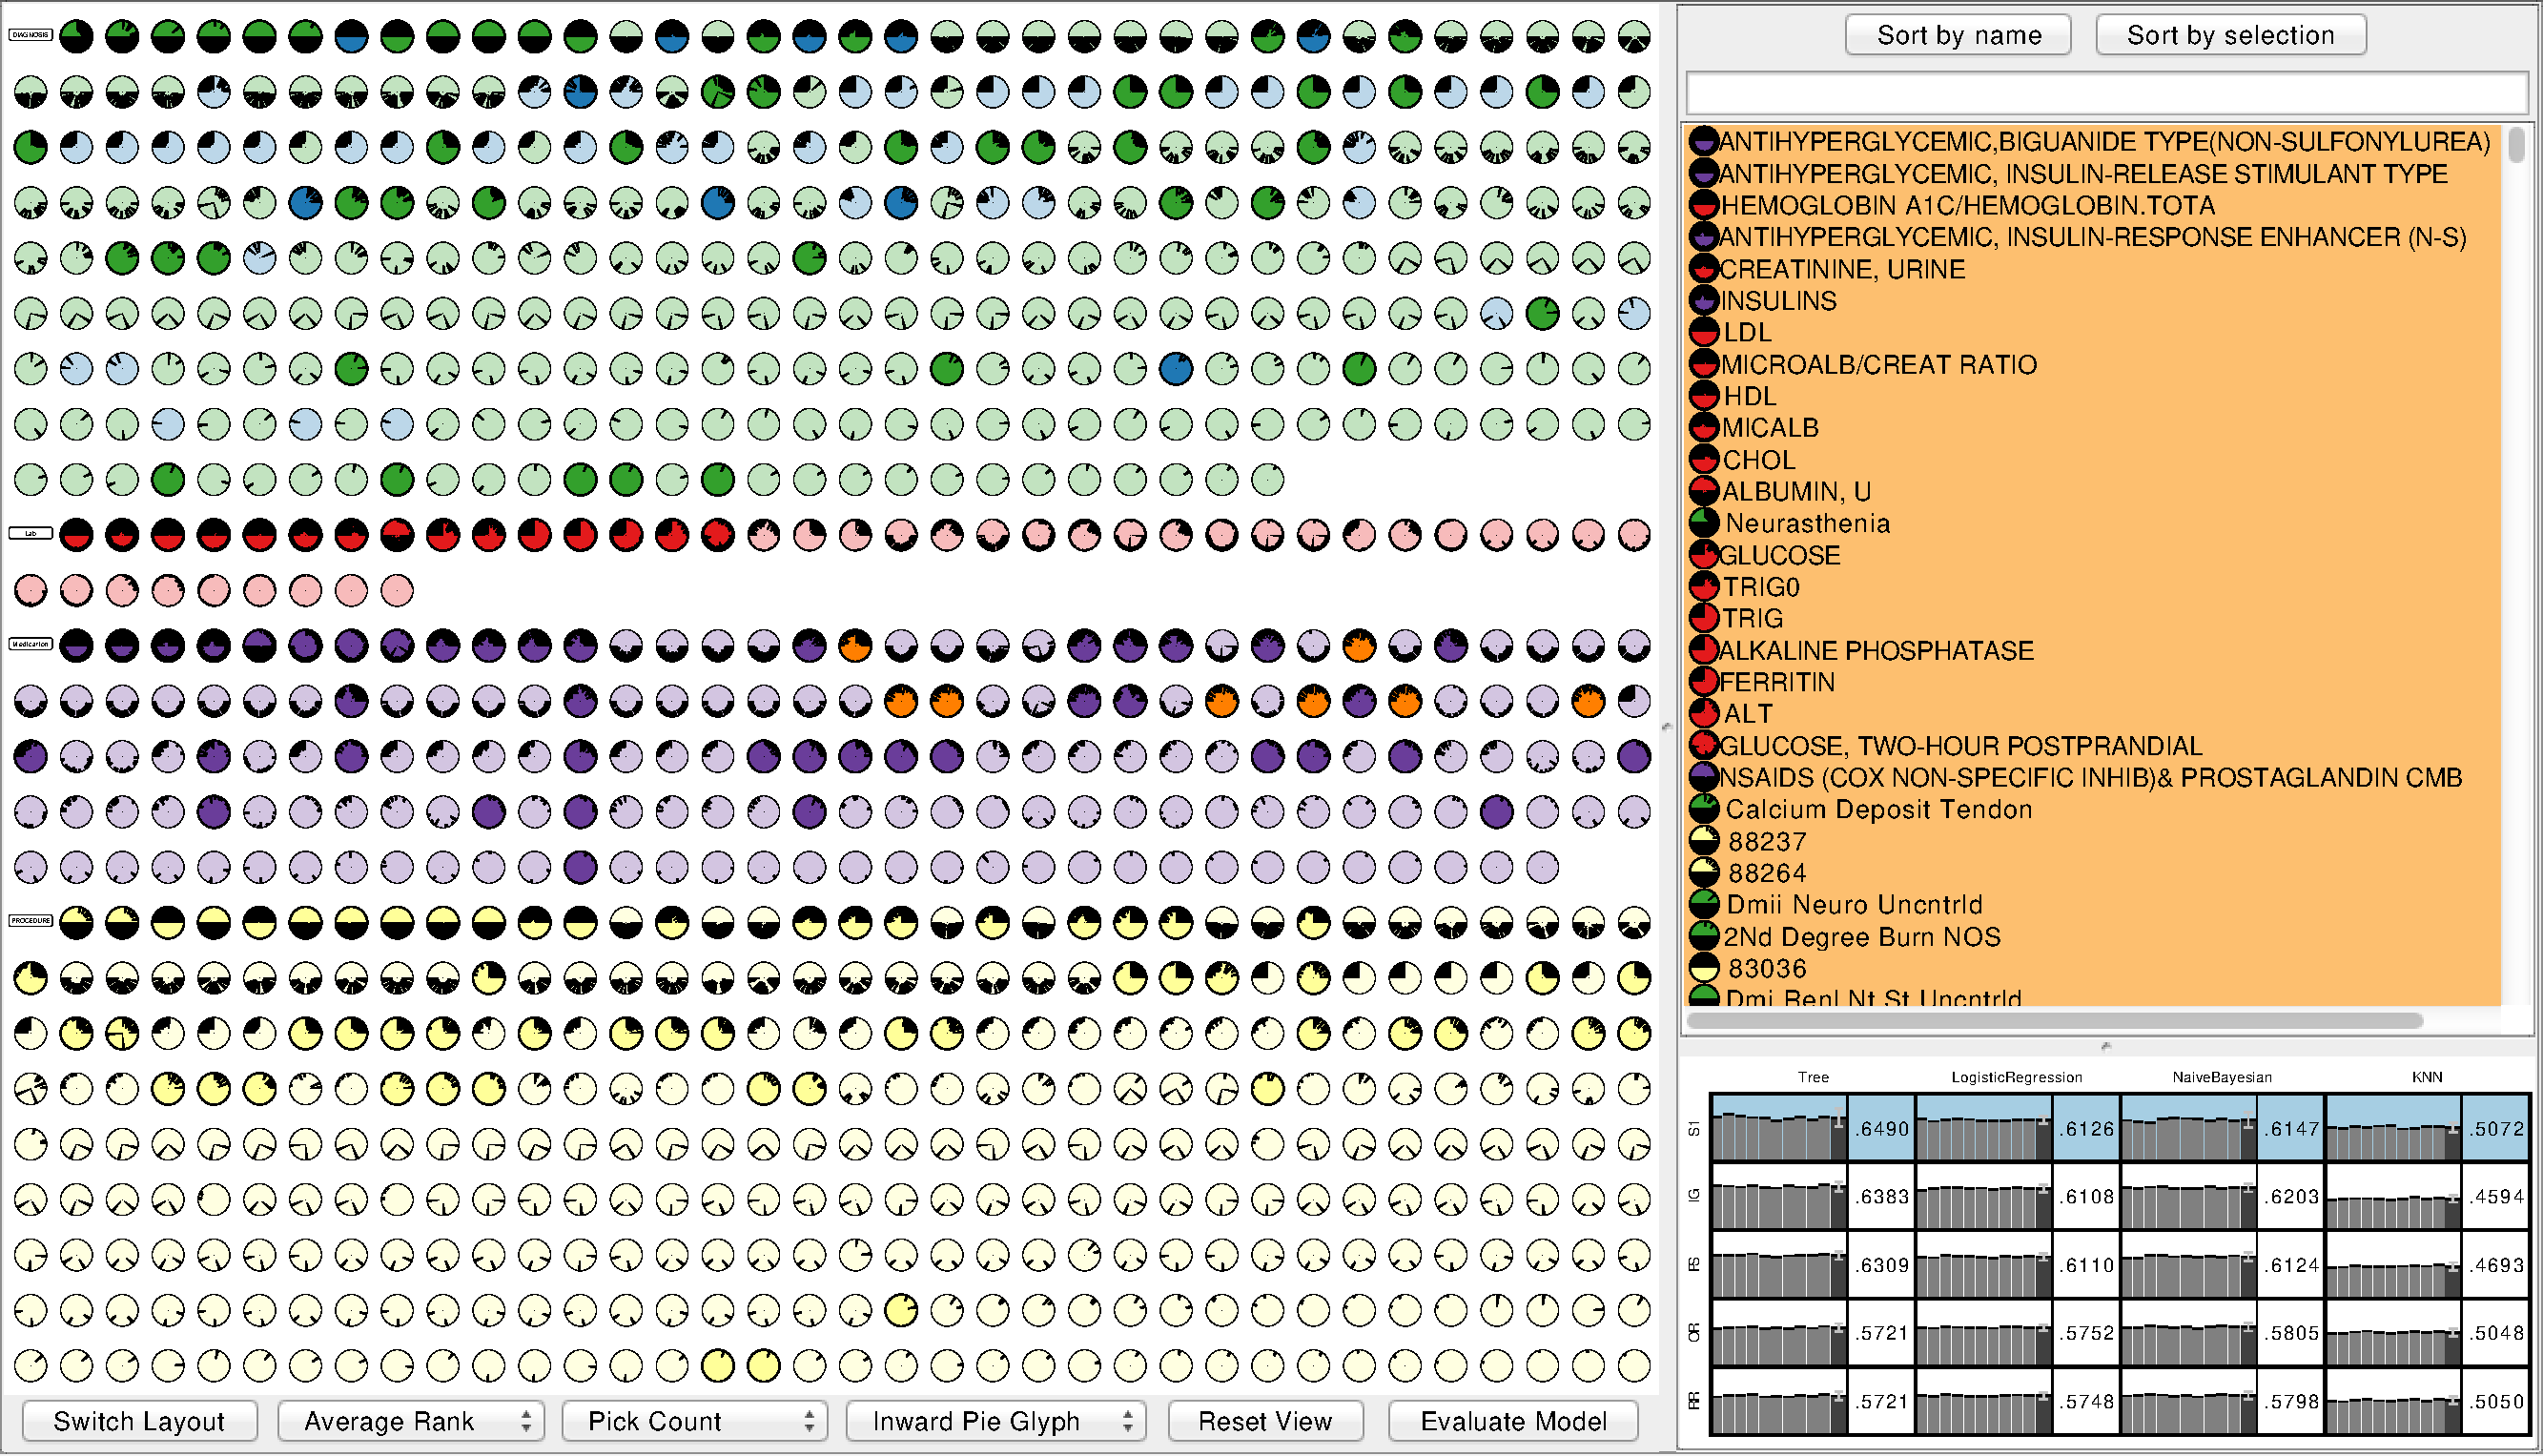
\includegraphics[width=\linewidth]{infuse/selection}
\caption[\infuse's Interactive Model Builder.]{
\infuse's Interactive Model Builder allows users to select sets of features and measure its quality.
Selected feature glyphs are highlighted by saturating their color.  The List View is sorted to show the selected features by their importance.  After a user has made their selections, they can evaluate their model by clicking the ``Evaluate Model" button.  This adds a new blue row to the the Classifier View, showing the results of the evaluation for the user-defined model.
}
\label{fig:selection}
\end{figure}

\subsection{Interactive Model Builder}
\label{sec:imb}

One of the most important aspects of \infuse is that in addition to allowing the comparison of models, it also enables the creation of new models based on insights.
Users can select features for model building in a variety of ways.  They can select all of the features from existing models by clicking on a model in the Classifier View.  This will highlight and select all of the features that were used in the model.  Users can then augment these lists, or start from an empty set, by selecting individual features when clicking on them in the Feature or List view.  In order to select multiple features, a lasso selection technique is available in the Ranked and Scatterplot layouts.

After a feature set has been collected, \infuse can automatically evaluate the predictive performance of the user-defined model. By clicking the ``Evaluate Model" button,
%(\adam{Would be better named as "Evaluate Selected Model" but may not be worth doing new screenshots})
the new model is scored across all cross-validation folds and classifiers, and the results are added in the Classifier panel as a new blue row.  In the example in Figure~\ref{fig:selection}, the user-defined model out-performed the automated models and it is ranked at the top of the Classifier View.
Note that the user created model does not appear in the glyph.
This is due to the fact that the user does not need to rank the
features in order to obtain a classification result and that the feature
set is equal for all cross-validation folds.

% In every part of the system, features can be selected.
% Entire groups of features can be selected via clicking on
% a model in the classifier view or by using lasso selection in
% the feature view.
% The selection of single features can be changed by clicking in
% either the feature or list view.
% The set of selected features can eventually be used
% to create a new model.
% By clicking on the rightmost button at the bottom
% the area under curve values for the new model are computed
% and a new row is inserted at the correct position in the classifier view
% (see Figure~\ref{fig:selection}).
% This is helpful for an expert to verify whether a manually created set of
% features performs better than the automatically created sets.
